\begin{figure}
\centering
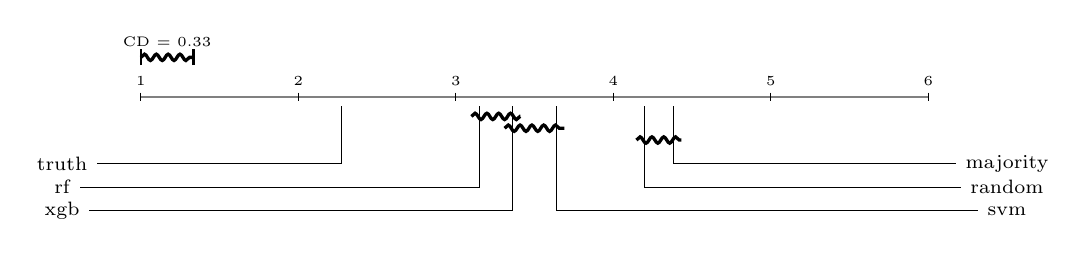
\begin{tikzpicture}[xscale=2]
\node (Label) at (1.1669470680467668, 0.7){\tiny{CD = 0.33}}; % the label
\draw[decorate,decoration={snake,amplitude=.4mm,segment length=1.5mm,post length=0mm},very thick, color = black] (1.0,0.5) -- (1.3338941360935335,0.5);
\foreach \x in {1.0, 1.3338941360935335} \draw[thick,color = black] (\x, 0.4) -- (\x, 0.6);

\draw[gray, thick](1.0,0) -- (6.0,0);
\foreach \x in {1.0,2.0,3.0,4.0,5.0,6.0} \draw (\x cm,1.5pt) -- (\x cm, -1.5pt);
\node (Label) at (1.0,0.2){\tiny{1}};
\node (Label) at (2.0,0.2){\tiny{2}};
\node (Label) at (3.0,0.2){\tiny{3}};
\node (Label) at (4.0,0.2){\tiny{4}};
\node (Label) at (5.0,0.2){\tiny{5}};
\node (Label) at (6.0,0.2){\tiny{6}};
\draw[decorate,decoration={snake,amplitude=.4mm,segment length=1.5mm,post length=0mm},very thick, color = black](3.0990196078431373,-0.25) -- (3.4098039215686273,-0.25);
\draw[decorate,decoration={snake,amplitude=.4mm,segment length=1.5mm,post length=0mm},very thick, color = black](3.3098039215686277,-0.4) -- (3.6892156862745096,-0.4);
\draw[decorate,decoration={snake,amplitude=.4mm,segment length=1.5mm,post length=0mm},very thick, color = black](4.147058823529412,-0.55) -- (4.432352941176471,-0.55);
\node (Point) at (2.272549019607843, 0){};\node (Label) at (0.5,-0.8500000000000001){\scriptsize{truth}}; \draw (Point) |- (Label);
\node (Point) at (3.149019607843137, 0){};\node (Label) at (0.5,-1.1500000000000001){\scriptsize{rf}}; \draw (Point) |- (Label);
\node (Point) at (3.3598039215686275, 0){};\node (Label) at (0.5,-1.4500000000000002){\scriptsize{xgb}}; \draw (Point) |- (Label);
\node (Point) at (4.382352941176471, 0){};\node (Label) at (6.5,-0.8500000000000001){\scriptsize{majority}}; \draw (Point) |- (Label);
\node (Point) at (4.197058823529412, 0){};\node (Label) at (6.5,-1.1500000000000001){\scriptsize{random}}; \draw (Point) |- (Label);
\node (Point) at (3.6392156862745098, 0){};\node (Label) at (6.5,-1.4500000000000002){\scriptsize{svm}}; \draw (Point) |- (Label);
\end{tikzpicture}
\caption{Nemenyi - input.csv}
\label{fig:nemenyi}
\end{figure}
